\documentclass[aspectratio=169]{beamer}
\usetheme{Madrid}
\usecolortheme{default}

% Packages
\usepackage[utf8]{inputenc}
\usepackage[T1]{fontenc}
\usepackage{graphicx}
\usepackage{booktabs}
\usepackage{amsmath}
\usepackage{amssymb}
\usepackage{listings}
\usepackage{xcolor}
\usepackage{tikz}
\usetikzlibrary{shapes.geometric, arrows, positioning}
\usepackage{pifont}
\newcommand{\cmark}{\ding{51}}
\newcommand{\xmark}{\ding{55}}

% Code styling
\lstset{
    basicstyle=\ttfamily\footnotesize,
    breaklines=true,
    frame=single,
    backgroundcolor=\color{gray!10}
}

% Title information
\title[Hybrid Financial Intelligence System]{Hybrid Financial Intelligence System}
\subtitle{ML-Based Stock Movement Prediction}
\author[Adimi \& Ben Amor]{Dalil ADIMI \and Hassen BEN AMOR}
\institute[EFREI Paris]{
    Group I2-NEW DAI \\
    Data Science Module \\
    \vspace{0.3cm}
    Supervisor: Stephany RAJEH \\
    EFREI Paris
}
\date{\today}

\begin{document}

% Title slide
\begin{frame}
    \titlepage
\end{frame}

% Outline
\begin{frame}{Outline}
    \tableofcontents
\end{frame}

% ============================================================
\section{Introduction}
% ============================================================

\begin{frame}{Project Overview}
    \begin{block}{Objective}
        Build an end-to-end ML pipeline that predicts whether a stock's price will rise by $>$3.5\% over the next 5 trading days (binary classification).
    \end{block}

    \vspace{0.4cm}

    \begin{columns}
        \column{0.5\textwidth}
        \textbf{Target Stocks:}
        \begin{itemize}
            \item SMCI (Super Micro Computer)
            \item CRSP (CRISPR Therapeutics)
            \item PLTR (Palantir Technologies)
        \end{itemize}

        \column{0.5\textwidth}
        \textbf{Tech Stack:}
        \begin{itemize}
            \item Python (pandas, scikit-learn, XGBoost)
            \item Plotly for visualization
            \item Streamlit dashboard
            \item FastAPI backend
        \end{itemize}
    \end{columns}
\end{frame}

% ============================================================
\section{Data Collection \& Preprocessing}
% ============================================================

\begin{frame}{Data Pipeline}
    \begin{columns}
        \column{0.55\textwidth}
        \textbf{Sources \& APIs:}
        \begin{table}
            \centering
            \small
            \begin{tabular}{ll}
                \toprule
                \textbf{Source} & \textbf{Library / API} \\
                \midrule
                Yahoo Finance & \texttt{yfinance} \\
                FRED & REST API \\
                Finnhub & REST API (optional) \\
                \bottomrule
            \end{tabular}
        \end{table}

        \vspace{0.2cm}
        \textbf{Dataset:}
        \begin{itemize}
            \item 4,414 daily records (2020--2026)
            \item 3 tickers, OHLCV + macro
            \item No missing values, no duplicates
        \end{itemize}

        \column{0.45\textwidth}
        \textbf{Preprocessing Steps:}
        \begin{enumerate}
            \item Download OHLCV per ticker
            \item Merge macro data (forward-fill)
            \item Compute 12 technical indicators
            \item Build 14-day rolling aggregates
            \item Generate binary target labels
            \item Drop NaN warm-up rows
        \end{enumerate}

        \vspace{0.2cm}
        \begin{block}{Result}
            4,357 rows $\times$ 40 columns
        \end{block}
    \end{columns}
\end{frame}

% ============================================================
\section{Exploratory Data Analysis}
% ============================================================

\begin{frame}{EDA --- Stock Prices}
    \begin{columns}
        \column{0.5\textwidth}
        % ---- PLACEHOLDER: insert normalized price chart ----
        \begin{center}
            \fbox{\parbox{0.9\textwidth}{\centering\vspace{2.5cm}\textit{[Insert: Normalized Price Chart]}\vspace{2.5cm}}}
        \end{center}

        \column{0.5\textwidth}
        \textbf{Observations:}
        \begin{itemize}
            \item SMCI: extreme rallies \& drawdowns
            \item PLTR: uptrend since late 2022
            \item CRSP: independent pattern
            \item Daily volatility: 3.8--5.2\%
        \end{itemize}

        \vspace{0.3cm}

        \textbf{Target Distribution:}
        \begin{itemize}
            \item Positive class (up $>$3.5\%): 34\%
            \item Negative class: 66\%
            \item Handled via \texttt{scale\_pos\_weight}
        \end{itemize}
    \end{columns}
\end{frame}

\begin{frame}{EDA --- Distributions \& Correlations}
    \begin{columns}
        \column{0.5\textwidth}
        % ---- PLACEHOLDER: insert return distribution plot ----
        \begin{center}
            \fbox{\parbox{0.9\textwidth}{\centering\vspace{2.5cm}\textit{[Insert: Return Distribution]}\vspace{2.5cm}}}
        \end{center}

        \column{0.5\textwidth}
        % ---- PLACEHOLDER: insert correlation heatmap ----
        \begin{center}
            \fbox{\parbox{0.9\textwidth}{\centering\vspace{2.5cm}\textit{[Insert: Correlation Heatmap]}\vspace{2.5cm}}}
        \end{center}
    \end{columns}
\end{frame}

% ============================================================
\section{Feature Engineering}
% ============================================================

\begin{frame}{Feature Engineering}
    \begin{columns}
        \column{0.5\textwidth}
        \textbf{12 Base Indicators:}
        \begin{itemize}
            \item RSI(14), MACD (line, signal, hist)
            \item Bollinger Band width
            \item Moving Averages (50, 200)
            \item ATR(14), ATR \%
            \item Volume Z-score
            \item 10Y Treasury Yield
        \end{itemize}

        \column{0.5\textwidth}
        \textbf{Rolling Window (14 days):}
        \begin{itemize}
            \item For each indicator: \textbf{mean, std, last}
            \item $12 \times 3 = 36$ features total
            \item Captures recent trend + variability
        \end{itemize}

        \vspace{0.3cm}

        \textbf{Target Variable:}
        \[
        y_t = \mathbb{1}\!\left(\frac{c_{t+5}}{c_t} - 1 > 0.035\right)
        \]
    \end{columns}

    \vspace{0.3cm}

    \begin{alertblock}{Why Rolling Windows?}
        Raw indicator values change scale over time. Rolling statistics normalize the features and improve generalization.
    \end{alertblock}
\end{frame}

% ============================================================
\section{Model Training \& Evaluation}
% ============================================================

\begin{frame}{Pipeline Architecture}
    \begin{center}
        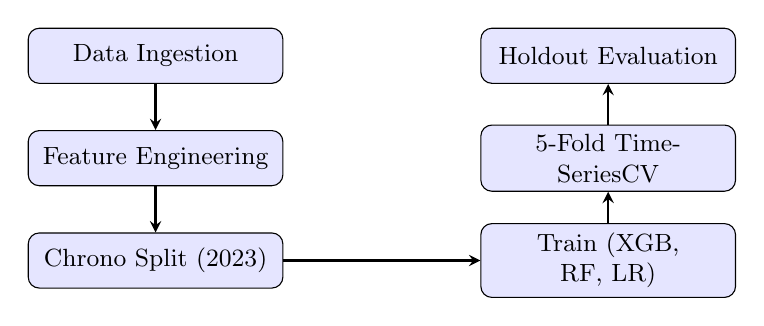
\begin{tikzpicture}[
            node distance=1.3cm,
            box/.style={rectangle, draw, fill=blue!10, text width=3cm, text centered, rounded corners, minimum height=0.7cm, font=\small},
            arrow/.style={->, >=stealth, thick}
        ]
            \node[box] (data) {Data Ingestion};
            \node[box, below of=data] (feat) {Feature Engineering};
            \node[box, below of=feat] (split) {Chrono Split (2023)};
            \node[box, right=2.5cm of split] (train) {Train (XGB, RF, LR)};
            \node[box, above of=train] (cv) {5-Fold TimeSeriesCV};
            \node[box, above of=cv] (eval) {Holdout Evaluation};

            \draw[arrow] (data) -- (feat);
            \draw[arrow] (feat) -- (split);
            \draw[arrow] (split) -- (train);
            \draw[arrow] (train) -- (cv);
            \draw[arrow] (cv) -- (eval);
        \end{tikzpicture}
    \end{center}

    \vspace{0.3cm}

    \begin{columns}
        \column{0.5\textwidth}
        \textbf{Train:} before 2023-01-01 (2,038 samples)\\
        \textbf{Test:} from 2023-01-01 (2,319 samples)

        \column{0.5\textwidth}
        \textbf{Scaling:} MinMaxScaler\\
        \textbf{CV metric:} Precision (5-fold)
    \end{columns}
\end{frame}

\begin{frame}{Model Comparison --- Results}
    \begin{table}
        \centering
        \begin{tabular}{lcccc}
            \toprule
            \textbf{Model} & \textbf{Accuracy} & \textbf{Precision} & \textbf{F1} & \textbf{ROC-AUC} \\
            \midrule
            XGBoost        & 53\% & 0.366 & 0.373 & 0.513 \\
            Random Forest  & 58\% & 0.390 & 0.303 & 0.518 \\
            Logistic Reg.  & 55\% & 0.399 & 0.406 & 0.506 \\
            \bottomrule
        \end{tabular}
    \end{table}

    \vspace{0.3cm}

    \begin{columns}
        \column{0.5\textwidth}
        % ---- PLACEHOLDER: insert confusion matrix ----
        \begin{center}
            \fbox{\parbox{0.85\textwidth}{\centering\vspace{2cm}\textit{[Insert: Confusion Matrix]}\vspace{2cm}}}
        \end{center}

        \column{0.5\textwidth}
        \textbf{Key Takeaways:}
        \begin{itemize}
            \item All models slightly above random (AUC $>$ 0.50)
            \item Logistic Regression competitive with tree models
            \item Stock prediction is inherently noisy --- these results are realistic
        \end{itemize}
    \end{columns}
\end{frame}

\begin{frame}{Backtest \& Equity Curve}
    \begin{columns}
        \column{0.5\textwidth}
        % ---- PLACEHOLDER: insert equity curve ----
        \begin{center}
            \fbox{\parbox{0.9\textwidth}{\centering\vspace{2.5cm}\textit{[Insert: Equity Curve]}\vspace{2.5cm}}}
        \end{center}

        \column{0.5\textwidth}
        \textbf{Backtest Setup:}
        \begin{itemize}
            \item Non-overlapping 5-day windows
            \item Long-only / cash strategy
            \item Signal: BUY if $P(\text{up}) \geq 0.50$
        \end{itemize}

        \vspace{0.3cm}

        \textbf{Metrics:}
        \begin{itemize}
            \item Annualized return: 31.3\%
            \item Max drawdown: $-$28.4\%
        \end{itemize}
    \end{columns}
\end{frame}

% ============================================================
\section{Deployment --- Dashboard}
% ============================================================

\begin{frame}{Live Dashboard}
    % ---- PLACEHOLDER: insert full dashboard screenshot ----
    \begin{center}
        \fbox{\parbox{0.85\textwidth}{\centering\vspace{4.5cm}\textit{[Insert: Dashboard Screenshot]}\vspace{4.5cm}}}
    \end{center}
\end{frame}

% ============================================================
\section{Conclusion \& Future Work}
% ============================================================

\begin{frame}{Conclusion}
    \textbf{What we built:}
    \begin{enumerate}
        \item End-to-end ML pipeline: ingestion $\rightarrow$ features $\rightarrow$ training $\rightarrow$ evaluation $\rightarrow$ deployment
        \item Chronological train/test split (no data leakage)
        \item 3 models compared (XGBoost, Random Forest, Logistic Regression)
        \item Streamlit dashboard + FastAPI for serving predictions
    \end{enumerate}

    \vspace{0.3cm}

    \textbf{Lessons learned:}
    \begin{itemize}
        \item Stock prediction is hard --- 53\% accuracy is realistic for this domain
        \item More features $\neq$ better performance (we tested 40+ features, marginal gain)
        \item Temporal validation is critical to avoid overfitting
        \item Simple, interpretable pipelines are more valuable than complex ones
    \end{itemize}
\end{frame}

\begin{frame}{Future Work}
    \begin{columns}
        \column{0.5\textwidth}
        \textbf{Model Improvements:}
        \begin{itemize}
            \item Add sentiment features (FinBERT)
            \item Try deep learning (LSTM, Transformers)
            \item Ensemble stacking
            \item Probability calibration
        \end{itemize}

        \column{0.5\textwidth}
        \textbf{Engineering:}
        \begin{itemize}
            \item Dockerized deployment
            \item Automated retraining pipeline
            \item Model monitoring \& drift detection
            \item CI/CD for model updates
        \end{itemize}
    \end{columns}
\end{frame}

% ============================================================
% Thank You
% ============================================================

\begin{frame}[plain]
    \begin{center}
        \Huge \textbf{Thank You!}

        \vspace{1.5cm}

        \LARGE Questions?

        \vspace{1.5cm}

        \large
        \textbf{Dalil ADIMI \& Hassen BEN AMOR}\\
        Group I2-NEW DAI --- EFREI Paris
    \end{center}
\end{frame}

\end{document}
